\subsubsection{The SolCx Stokes benchmark}
\label{sec:benchmark-solcx}

The SolCx benchmark is intended to test the accuracy of the solution to a
problem that has a large jump in the viscosity along a line through the
domain. Such situations are common in geophysics: for example, the viscosity
in a cold, subducting slab is much larger than in the surrounding, relatively
hot mantle material.

The SolCx benchmark computes the Stokes flow field of a fluid driven by
spatial density variations, subject to a spatially variable
viscosity. Specifically, the domain is $\Omega=[0,1]^2$, gravity is $\mathbf
g=(0,-1)^T$ and the density is given
by $\rho(\mathbf x)=\sin(\pi x_1)\cos(\pi x_2)$; this can be considered a
density perturbation to a constant background density. The viscosity is
\begin{align*}
  \eta(\mathbf x) = \left\{
    \begin{matrix}
      1 & \text{for}\ x_1 \le 0.5, \\
      10^6 & \text{for}\ x_1  > 0.5.
    \end{matrix}
  \right.
\end{align*}
This strongly discontinuous viscosity field yields an almost stagnant flow in
the right half of the domain and consequently a singularity in the pressure
along the interface.
Boundary conditions are free slip on all of $\partial\Omega$. The temperature
plays no role in this benchmark. The prescribed density field and the
resulting velocity field are shown in Fig.~\ref{fig:solcx}.

The SolCx benchmark was previously used in \cite[Section 4.1.1]{DMGT11}
(references to earlier uses of the benchmark are available there) and its analytic
solution is given in \cite{Zho96}. \aspect{} contains an implementation of
this analytic solution taken from the Underworld package (see \cite{MQLMAM07}
and \url{http://www.underworldproject.org/}, and correcting for the mismatch
in sign between the implementation and the description in \cite{DMGT11}).

\begin{figure}
  \begin{center}
    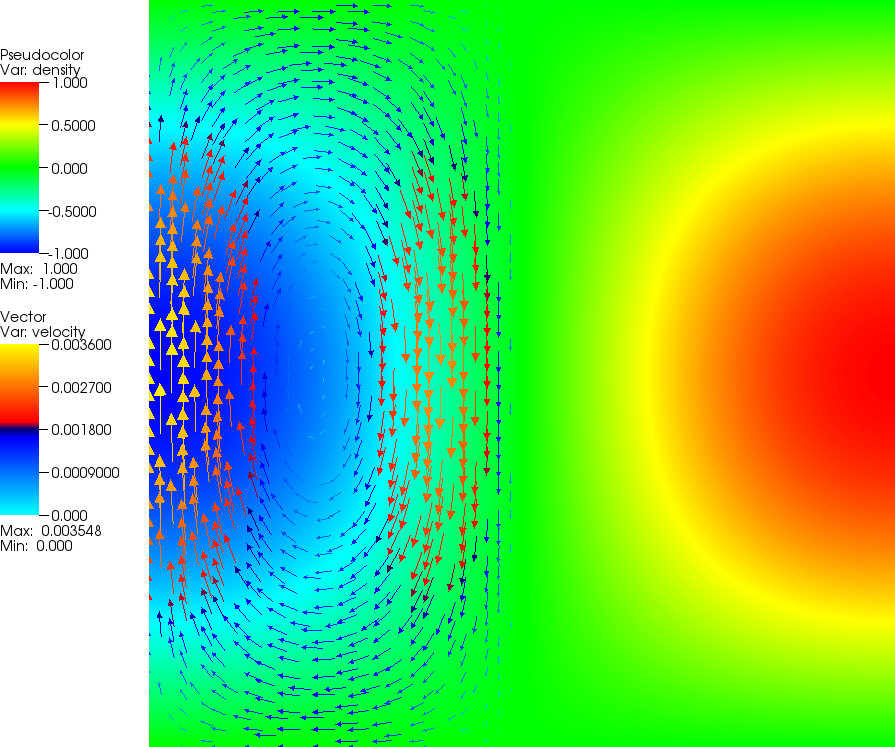
\includegraphics[width=0.45\textwidth]{cookbooks/benchmarks/solcx/doc/solcx-solution.png}
    \hfill
    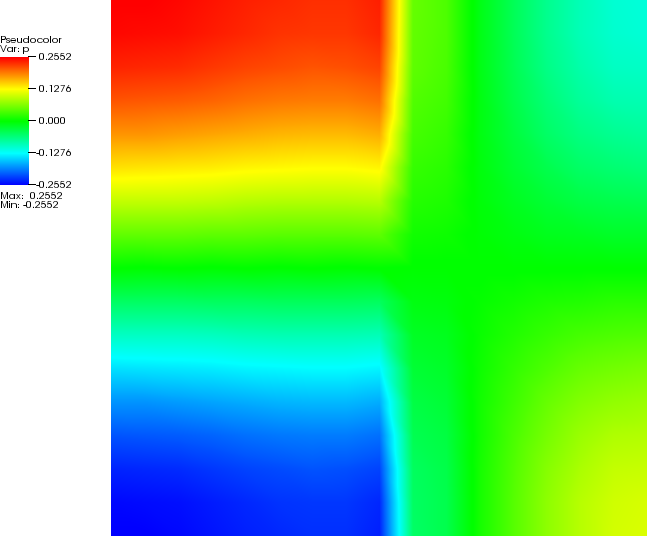
\includegraphics[width=0.45\textwidth]{cookbooks/benchmarks/solcx/doc/solcx-solution-pressure.png}
    \caption{\it SolCx Stokes benchmark. Left: The density perturbation field
    and overlaid to it some velocity vectors. The viscosity is very large in the
      right hand, leading to a stagnant flow in this region. Right: The
      pressure on a relatively coarse mesh, showing the internal layer along
      the line where the viscosity jumps.}
    \label{fig:solcx}
  \end{center}
\end{figure}

To run this benchmark, the following input file will do (see the files in \url{benchmarks/solcx/} to rerun the benchmark):
\lstinputlisting[language=prmfile]{cookbooks/benchmarks/solcx/doc/solcx.prm.out}

Since this is the first cookbook in the benchmarking section, let us go
through the different parts of this file in more detail:
\begin{itemize}
\item The material model and the postprocessor
\item The first part consists of parameter setting for overall
  parameters. Specifically, we set the dimension in which this benchmark runs
  to two and choose an output directory. Since we are not interested in a time
  dependent solution, we set the end time equal to the start time, which
  results in only a single time step being computed.

  The last parameter of this section, \texttt{Pressure normalization},
\index[prmindex]{Pressure normalization}
\index[prmindexfull]{Pressure normalization}
  is set in such a way that the pressure is chosen so that its \textit{domain}
  average is zero, rather than the pressure along the surface, see
  Section~\ref{sec:pressure}.

\item The next part of the input file describes the setup of the
  benchmark. Specifically, we have to say how the geometry should look like (a
  box of size $1\times 1$) and what the velocity boundary conditions shall be
  (tangential flow all around -- the box geometry defines four boundary
\index[prmindex]{Model name}
\index[prmindexfull]{Geometry model!Model name}
  indicators for the left, right, bottom and top boundaries, see also
  Section~\ref{parameters:Geometry_20model}). This is followed by subsections
  choosing the material model (where we choose a particular model implemented
  in \aspect{} that describes the spatially variable density and viscosity
  fields, along with the size of the viscosity jump) and finally the chosen
  gravity model (a gravity field that is the constant vector $(0,-1)^T$, see
\index[prmindex]{Model name}
\index[prmindexfull]{Gravity model!Model name}
  Section~\ref{parameters:Gravity_20model}).

\item The part that follows this describes the boundary and initial values for
  the temperature. While we are not interested in the evolution of the
  temperature field in this benchmark, we nevertheless need to set
  something. The values given here are the minimal set of inputs.

\item The second-to-last part sets discretization parameters. Specifically, it
  determines what kind of Stokes element to choose (see
\index[prmindex]{Stokes velocity polynomial degree}
\index[prmindexfull]{Discretization!Stokes velocity polynomial degree}
  Section~\ref{parameters:Discretization} and the extensive discussion in
  \cite{KHB12}). We do not adaptively refine the mesh but only do four global
  refinement steps at the very beginning. This is obviously a parameter worth
\index[prmindex]{Initial global refinement}
\index[prmindexfull]{Mesh refinement!Initial global refinement}
  playing with.

\item The final section on postprocessors determines what to do with the
  solution once computed. Here, we do two things: we ask \aspect{} to compute
  the error in the solution using the setup described in the Duretz et
  al.~paper \cite{DMGT11}, and we request that output files for later
  visualization are generated and placed in the output directory. The
  functions that compute the error automatically query which kind of material
  model had been chosen, i.e., they can know whether we are solving the SolCx
  benchmark or one of the other benchmarks discussed in the following
  subsections.
\end{itemize}

Upon running \aspect{} with this input file, you will get output of the
following kind (obviously with different timings, and details of the output
may also change as development of the code continues):
\begin{lstlisting}[frame=single,language=ksh]
aspect/cookbooks> ../aspect solcx.prm
Number of active cells: 256 (on 5 levels)
Number of degrees of freedom: 3,556 (2,178+289+1,089)

*** Timestep 0:  t=0 years
   Solving temperature system... 0 iterations.
   Rebuilding Stokes preconditioner...
   Solving Stokes system... 30+3 iterations.

   Postprocessing:
     Errors u_L1, p_L1, u_L2, p_L2: 1.125997e-06, 2.994143e-03, 1.670009e-06, 9.778441e-03
     Writing graphical output:      output/solution/solution-00000



+---------------------------------------------+------------+------------+
| Total wallclock time elapsed since start    |      1.51s |            |
|                                             |            |            |
| Section                         | no. calls |  wall time | % of total |
+---------------------------------+-----------+------------+------------+
| Assemble Stokes system          |         1 |     0.114s |       7.6% |
| Assemble temperature system     |         1 |     0.284s |        19% |
| Build Stokes preconditioner     |         1 |    0.0935s |       6.2% |
| Build temperature preconditioner|         1 |    0.0043s |      0.29% |
| Solve Stokes system             |         1 |    0.0717s |       4.8% |
| Solve temperature system        |         1 |  0.000753s |      0.05% |
| Postprocessing                  |         1 |     0.627s |        42% |
| Setup dof systems               |         1 |      0.19s |        13% |
+---------------------------------+-----------+------------+------------+
\end{lstlisting}

One can then visualize the solution in a number of different ways (see
Section~\ref{sec:viz}), yielding pictures like those shown in
Fig.~\ref{fig:solcx}. One can also analyze the error as shown in various
different ways, for example as a function of the mesh refinement level, the
element chosen, etc.; we have done so extensively in \cite{KHB12}.
